% !TEX encoding = UTF-8 Unicode
\documentclass[11pt]{article}

\usepackage[utf8x]{inputenc}
\usepackage[frenchb]{babel}
\usepackage[T1]{fontenc}
\usepackage{lmodern}
\usepackage{fullpage}
\usepackage{graphicx}
\usepackage{epstopdf}
\usepackage{caption}
\usepackage{subcaption}
\usepackage{multirow}
\pagestyle{plain}

% Math symbols
\usepackage{amsmath}
\usepackage{amssymb}
\usepackage{amsthm}

% Numbers and units
\usepackage[squaren, Gray]{SIunits}
\usepackage{sistyle}
\usepackage[autolanguage]{numprint}
%\usepackage{numprint}
\newcommand\si[2]{\numprint[#2]{#1}}
\newcommand\np[1]{\numprint{#1}}

\DeclareMathOperator{\newdiff}{d} % use \dif instead
\newcommand{\dif}{\newdiff\!}
\newcommand{\fpart}[2]{\frac{\partial #1}{\partial #2}}
\newcommand{\ffpart}[2]{\frac{\partial^2 #1}{\partial #2^2}}
\newcommand{\fdpart}[3]{\frac{\partial^2 #1}{\partial #2\partial #3}}
\newcommand{\fdif}[2]{\frac{\dif #1}{\dif #2}}
\newcommand{\ffdif}[2]{\frac{\dif^2 #1}{\dif #2^2}}
\newcommand{\constant}{\ensuremath{\mathrm{cst}}}
\DeclareMathOperator{\im}{Im}

% Color
% cfr http://en.wikibooks.org/wiki/LaTeX/Colors
\usepackage{color}
\usepackage[usenames,dvipsnames,svgnames,table]{xcolor}
\definecolor{dkgreen}{rgb}{0.25,0.7,0.35}
\definecolor{dkred}{rgb}{0.7,0,0}

% Listing
\usepackage{listings}
\lstset{
  numbers=left,
  numberstyle=\tiny\color{gray},
  basicstyle=\rm\small\ttfamily,
  keywordstyle=\bfseries\color{dkred},
  frame=single,
  commentstyle=\color{gray}=small,
  stringstyle=\color{dkgreen},
  %backgroundcolor=\color{gray!10},
  %tabsize=2,
  rulecolor=\color{black!30},
  %title=\lstname,
  breaklines=true,
  framextopmargin=2pt,
  framexbottommargin=2pt,
  extendedchars=true,
  inputencoding=utf8x,
  language=Matlab
}

\title{LINMA1170 -- Numerical Analysis I -- Homework 1\\ \normalsize{Prof. : P. Van Dooren. Teaching assistant: P.-A. Beaufort.}\\ }
\author{ Robin Libois -- 37581200 \\ Louis Regout -- 86291400 \\ Julien Vaes -- 80291100 \\ Levi Tinel --}
\date{\today}
\begin{document}
\maketitle



\section*{Echauffement}
Il nous est demandé de déterminer la suite de Sturm  $(f_0(x), \, f_1(x),\, \dots, \, f_m(x))$
pour le polynôme $f_0(x) = x^4 + 3x^2 +2$.
Pour déterminer cette dernière, il suffit d'appliquer la définition donnée à
la page 2 du syllabus c-à-d:
\begin{eqnarray}
  f_1(x) &=& f_0'(x)\\
  f_i(x) &=& q_{i+1}(x)f_{i+1}(x)-f_{i+2}(x), \quad i = 0, \dots, m-2; \label{eqDef} \\
  f_{m-1}(x)&=&q_{m}(x)f_{m}.
\end{eqnarray}

Ceci nous donne donc $f_{1}(x) = 4x^3 + 6x$. Pour les termes suivants de la suite il est nécessaire de
résoudre l'équation \ref{eqDef}. Nous allons illustrer la manière de procéder pour déterminer $f_{2}(x)$, les termes suivants de la suite
se calculent de manière identique. D'après \ref{eqDef}, il est nécessaire que $f_{2}(x)$ satifasse :
\begin{eqnarray}
   f_{0}(x)&=&q_{1}(x)f_{1}(x)-f_{2}(x)\\
   x^4 + 3x^2 +2 &=& (4x^3 + 6x)(a_0 + a_1x) - (r_0+r_1x+r_2x^2+r_3x^3) \label{initSyst}
\end{eqnarray}
Il est a noter que le reste de la division est d'au moins un degré inférieur à celui de $f_{0}(x)$. D'autre part, dans cette division ci, $q_1 (x)$
est de degré maximum égal à 1. Le quotient et le reste s'obtiennent aisément en appliquant la devision euclidienne\footnote{la division eulidienne donne $f (x) = q (x) d (x) + r (x)$,
or dans la récurrence nous désirons ${\color{red}-}r (x)$. Il faut donc inverser le signes du reste.} :

$$
\begin{array}{rrrrr|ll}
 x^4&&+3x^2&&+2 &4x^3+6x  &  \\
\cline{6-7}
 \color{blue}{x^4}&& \color{blue}{+\frac{3}{2}x^2}&& & \color{blue}{\frac{x}{4}} &   \\
\cline{1-3}
&&\frac{6x^2}{4}&&+2&&
\end{array}
$$
Nous en déduisons donc que $f_{2}(x)=\frac{-3x^2}{2}-2$ et $q_{1}(x)=\frac{x}{4}$. Si on applique la même méthode pour les autres polynômes
de la suite de Sturm nous obtenons :

\begin{center}
  \begin{tabular}{|l|l|}
    \hline
    $f_{0}(x)=x^4+3x^2+2$&\\
    $f_1 (x) = 4x^3+6x$&$q_1 (x) = \frac{x}{4}$\\
    $f_2 (x) = \frac{-3x^2}{2}-2$&$q_2 (x) = \frac{-8x}{3}$\\
    $f_3 (x) = \frac{-2x}{3}$&$q_3 (x)=\frac{9x}{4}$\\
    $f_4 (x)=2$&$q_4 (x) = \frac{-x}{3}$\\
    \hline
  \end{tabular}\hspace{1cm}\begin{tabular}{c||c|c|c|c|c||c}
      &$f_0$&$f_1$&$f_2$&$f_3$&$f_4$&$V (x)$\\
      \hline
      $-\infty$&+&-&-&+&+&2\\
      $\infty$&+&+&-&-&+&2\\
    \end{tabular}
\end{center}

D'après le théorème de Sturm, $N(\alpha,\beta)$ determine le nombre de racines réelles distinctes
du polynôme $f_{0} (x)$ comprises entre $\alpha$ et $\beta$. Dans notre cas $V(-\infty)=2$ et $V(+\infty)=2$,
nous en concluons que $f_{0} (x)$ ne possède pas de racines réelles et par conséquent possède deux pairs
de racines complexes conjuguées.
\section*{Mise en oeuvre}

\begin{itemize}
  \item [\textbullet] À l'aide de la fonction \textit{algEuclide}, nous obtenons que $V=0$ pour des valeurs de $\alpha=-\infty$ et $\beta = + \infty$.
  Tout comme dans la partie échauffement, nous pouvons conclure que $f_{0}(x)$ ne possède pas de racines réelles. Or comme les coefficients du
  polynôme sont réels, cela implique que les racines de $f_{0}(x)$ sont complexes conjuguées : $r_{1,2}=a\pm bi$ et $r_{3,4}=c\pm di$.
  \item [\textbullet] Il nous est demandé de caratériser les racines du polynômes $f_0(x)=x^{11} −10x^9 −7x^8 +27x^7 +70x^6 −20x^5 −189x^4 +50x^3 +140x^2 −350$.
  L'algortihme d'Euclide fournit le polynome suivant : $f_{m}(x)=10^6\cdot(-0.9700x^2+4.8502)$. De plus nous avons que $N(-\infty, 0)=1$ et $N(0,+\infty)=2$. Nous en déduisons donc que $f_0 (x)$
  possède trois racines réelles distinctes dont deux sont positives et l'une est négative. \\

  D'autre part, puisque $f_m (x)$ est non constant et qu'il est le pgcd de $f_0 (x)$ et $f_1 (x)$, toute racine de $f_m (x)$ est au moins une racine double de $f_0 (x)$.
  L'algortihme d'Euclide appliqué à $f_m (x)$ fournit le polynome suivant : $h_{m}(x)=(-4.8502)\cdot10^6$. Ainsi comme $h_{m}(x)$ est un polynôme
  constant, chaque racine de $f_m (x)$ est simple. De plus, pour  $f_m (x)$  nous avons $N(-\infty, 0)=1$ et $N(0,+\infty)=1$, ce qui implique que  $f_m (x)$
  possède une racine positive et une négative. Ainsi $f_{0}(x)$ possède deux racines réelles doubles : une négative et une autre positive. \\

  En conclusion les racines réelles de $f_{0}(x)$ peuvent être caractérisées de la manière suivante :\\

  \begin{center}
    \begin{tabular}{|c||c|c|}
      \hline
      Racine&Signe&Multiplicité\\
      \hline
      \hline
      \textbf{1)}&-&2\\
      \hline
      \textbf{2)}&+&1\\
      \hline
      \textbf{3)}&+&2\\
      \hline
    \end{tabular}
  \end{center}
\end{itemize}

\clearpage
\section*{Réflexion}
Soit le polynôme $f_n(x) = a_n x^{n} + a_{n-1}x^{n-1} + a_{n-2}x^{n-2}+\dots + a_1x+a_0$ de degré $n$. Afin de démontrer que le tableau de Routh d'un polynôme
peut être généré par l'algorithme d'Euclide : considérons pour cela les polynômes suivants :
\begin{eqnarray}
  P_n(x)&=& a_nx^n-a_{n-2}x^{n-2}+a_{n-4}x^{n-4}-\dots\\
  P_{n-1}(x)&=& a_{n-1}x^{n-1}-a_{n-3}x^{n-3}+a_{n-5}x^{n-5}-\dots\\
\end{eqnarray}
A l'aide de l'algorithme d'Euclide, il est possible de trouver un polynôme $P_{n-2} (x) = b_{1}x^{n-2}-b_{2}x^{n-4}+\dots$ où
\begin{eqnarray}
  P_n (x)   &=& \color{blue}{Q_{n-1}(x)} \color{black}P_{n-1}(x)-P_{n-2}(x) \nonumber\\
  \Leftrightarrow P_{n-2}(x) &=& \color{blue}\frac{a_n}{a_{n-1}}x\color{black} \cdot P_{n-1}(x) - P_{n} \nonumber\\
  \Leftrightarrow P_{n-2}(x) &=& \frac{a_n x P_{n-1}(x) - a_{n-1}P_n}{a_n} \label{equCoefP3}
\end{eqnarray}
Ainsi d'après (\ref{equCoefP3}), nous obtenons que $b_1 = \frac{a_{n-2}a_{n-1}-a_n a_{n-3}}{a_{n-1}}$,
$b_2 = \frac{a_{n-4}a_{n-1}-a_n a_{n-5}}{a_{n-1}}$, $\dots$. On en déduit que $b_i = \frac{a_{n-2i}a_{n-1}-a_n a_{n-2i-1}}{a_{n-1}}$.
Obtenons maintenant le polyôme $P_{n-3}(x) = c_1x^{n-3}-c_3x^{n-5}+\dots$ comme étant le reste de la division de $P_{n-1}(x)$ avec $P_{n-2}(x)$ :
\begin{eqnarray}
  P_{n-1} (x)   &=& \color{blue}{Q_{n-2}(x)} \color{black}P_{n-2}(x)-P_{n-3}(x) \nonumber\\
  \Leftrightarrow P_{n-3}(x) &=& \color{blue}\frac{a_{n-1}}{b_1}x\color{black} \cdot P_{n-2}(x) - P_{n-1} \nonumber\\
  \Leftrightarrow P_{n-3}(x) &=& \frac{a_{n-1} x P_{n-2}(x) - b_1P_{n-1}}{b_1}
\end{eqnarray}
Ce qui nous donne que $c_i = \frac{b_1a_{n-2i-1}-b_{i+1}a_{n-1}}{b_1}$.
De manière identique le polyôme $P_{n-4}(x) = d_1x^{n-4}-d_2x^{n-6}+\dots$ est le reste de la division de $P_{n-2}(x)$ avec $P_{n-3}(x)$ :
\begin{eqnarray}
  P_{n-2} (x)   &=& \color{blue}{Q_{n-3}(x)} \color{black}P_{n-3}(x)-P_{n-4}(x) \nonumber\\
  \Leftrightarrow P_{n-4}(x) &=& \color{blue}\frac{b_1}{c_1}x\color{black} \cdot P_{n-3}(x) - P_{n-2} \nonumber\\
  \Leftrightarrow P_{n-4}(x) &=& \frac{b_1 x P_{n-3}(x) - c_1P_{n-2}}{c_1}
\end{eqnarray}
Ce qui nous donne que $d_i = \frac{c_1b_{i+1}-b_1c_{i+1}}{c_1}$. Et ainsi de suite ...\\


En conclusion, il est possible de definir facilement le tableau de Routh d'un polynôme à coefficients
réels à l'aide de l'algorithme d'Euclide. En effet si nous définissions $P_n (x)$ et $P_{n-1} (x)$ comme precédement
 et si nous considérons la récurrence $P_i (x) = P_{i-1}(x) Q_{i-1}(x) - P_{i-2}(x)$ pour $i=0,\dots,m-2$, nous pouvons affirmer que l'élément $t_{i,j}$ du tableau
 de Routh est égal à $(-1)^{j+1} \mathbf{a_j}(P_{n-i+1})$ où $\mathbf{a_j}(P_{n-i+1})$ est le $j^{\text{ième}}$ coefficient non nul du polynôme $P_{n-i+1}(x)$ (en regardant les coefficients du degré le plus élévé au moins élevé).
 Par exemple, $\mathbf{a_2}(P_{n}) = -a_{n-2}$ ainsi $t_{1,2} = a_{n-2}$.

\clearpage

\section*{Performances}

\textbf{Remarque :} pour l'étude des performances, nous avons forcé Matlab a n'utiliser qu'un seul \textit{thread}.

\paragraph{Complexité théorique de notre fonction} Dans notre fonction \textit{AlgEuclide}, une boucle \textit{while} effectue la division euclidienne. Dans le pire des cas $n$ divisions euclidiennes
    devront être calculées, et donc $n$ itérations seront nécesssaires. La division euclidienne de polynômes se fait en $\mathcal{O}(n)$.
    De plus à l'intérieur de cette même boucle les fonctions \textit{makeTrueZero}\footnote{fonction qui transforme des petites valeurs ($<10^{-10}$) en 0.} et \textit{signeVec}\footnote{Fonction qui transforme un vecteur $v$ de la manière suivante : si $v(i)<0$ alors $v(i)=-1$, si $v(i)=0$ alors $v(i)=0$ et enfin si $v(i)>0$ alors $v(i)=1$.} ont toutes les deux une complexité en $\matcal{O}(n)$.
     Ainsi nous pouvons déduire que la complexité temporelle théorique de AlgEuclide est de $\mathcal{O}(n^2)$. En effet

    $$\Rightarrow Complexité = \mathcal{O}(n*(n+n+n)) = \mathcal{O}(3*n^2) = \mathcal{O}(n^2) $$

\paragraph{Complexité pratique de notre fonction}
    Pour vérifier la complexité théorique trouvée de \textit{AlgEuclide}, nous avons mesuré son temps d'exécution en fonction du degré $n$ de $f_0$.

    \begin{center}
      \begin{tabular}{|l|l|l|l|l|l|l|l|l|l|l|}
  \hline
      Degré de $f_0$ & 1000 & 1500 & 2000 & 2500 & 3000 & 3500 & 4000 & 4500 & 5000 \\
      \hline
     Temps d'éxécution (ms) & 14 & 24 & 34 & 50 & 65 & 173 & 101 & 132 & 146\\
     \hline
  \end{tabular}
    \end{center}

    Sur le graphe log-log suivant est représenté le temps necesssaire en fonction du degré du polynôme.
    Nous savons que si $d$ est la pente de la regression linéaire, alors expérimentalement notre fonction aura
    une complexité de $\mathcal{O}(n^d)$. En effet si nous supposons que la complexité est en $\mathcal{O}(n^k)$, $k$ est obtenu
    par la pente de la regression :
    $$ pente = \frac{log(Cn_1^k)-log(Cn_0^k)}{log(n_1)-log(n_0)} = k, $$
    où $n_0$, $n_1$ sont des entiers représentant le dégré des polynômes et $C$ est la constante lié à la complexité.\\

    Nous avons distingué deux cas : à gauche les coeffients sont entiers pris aléatoirement
    entre 0 et 10, à droite les coefficients valent 1. Ce second cas est moins bien conditionné et devrait prendre plus de temps.

        \begin{center}
          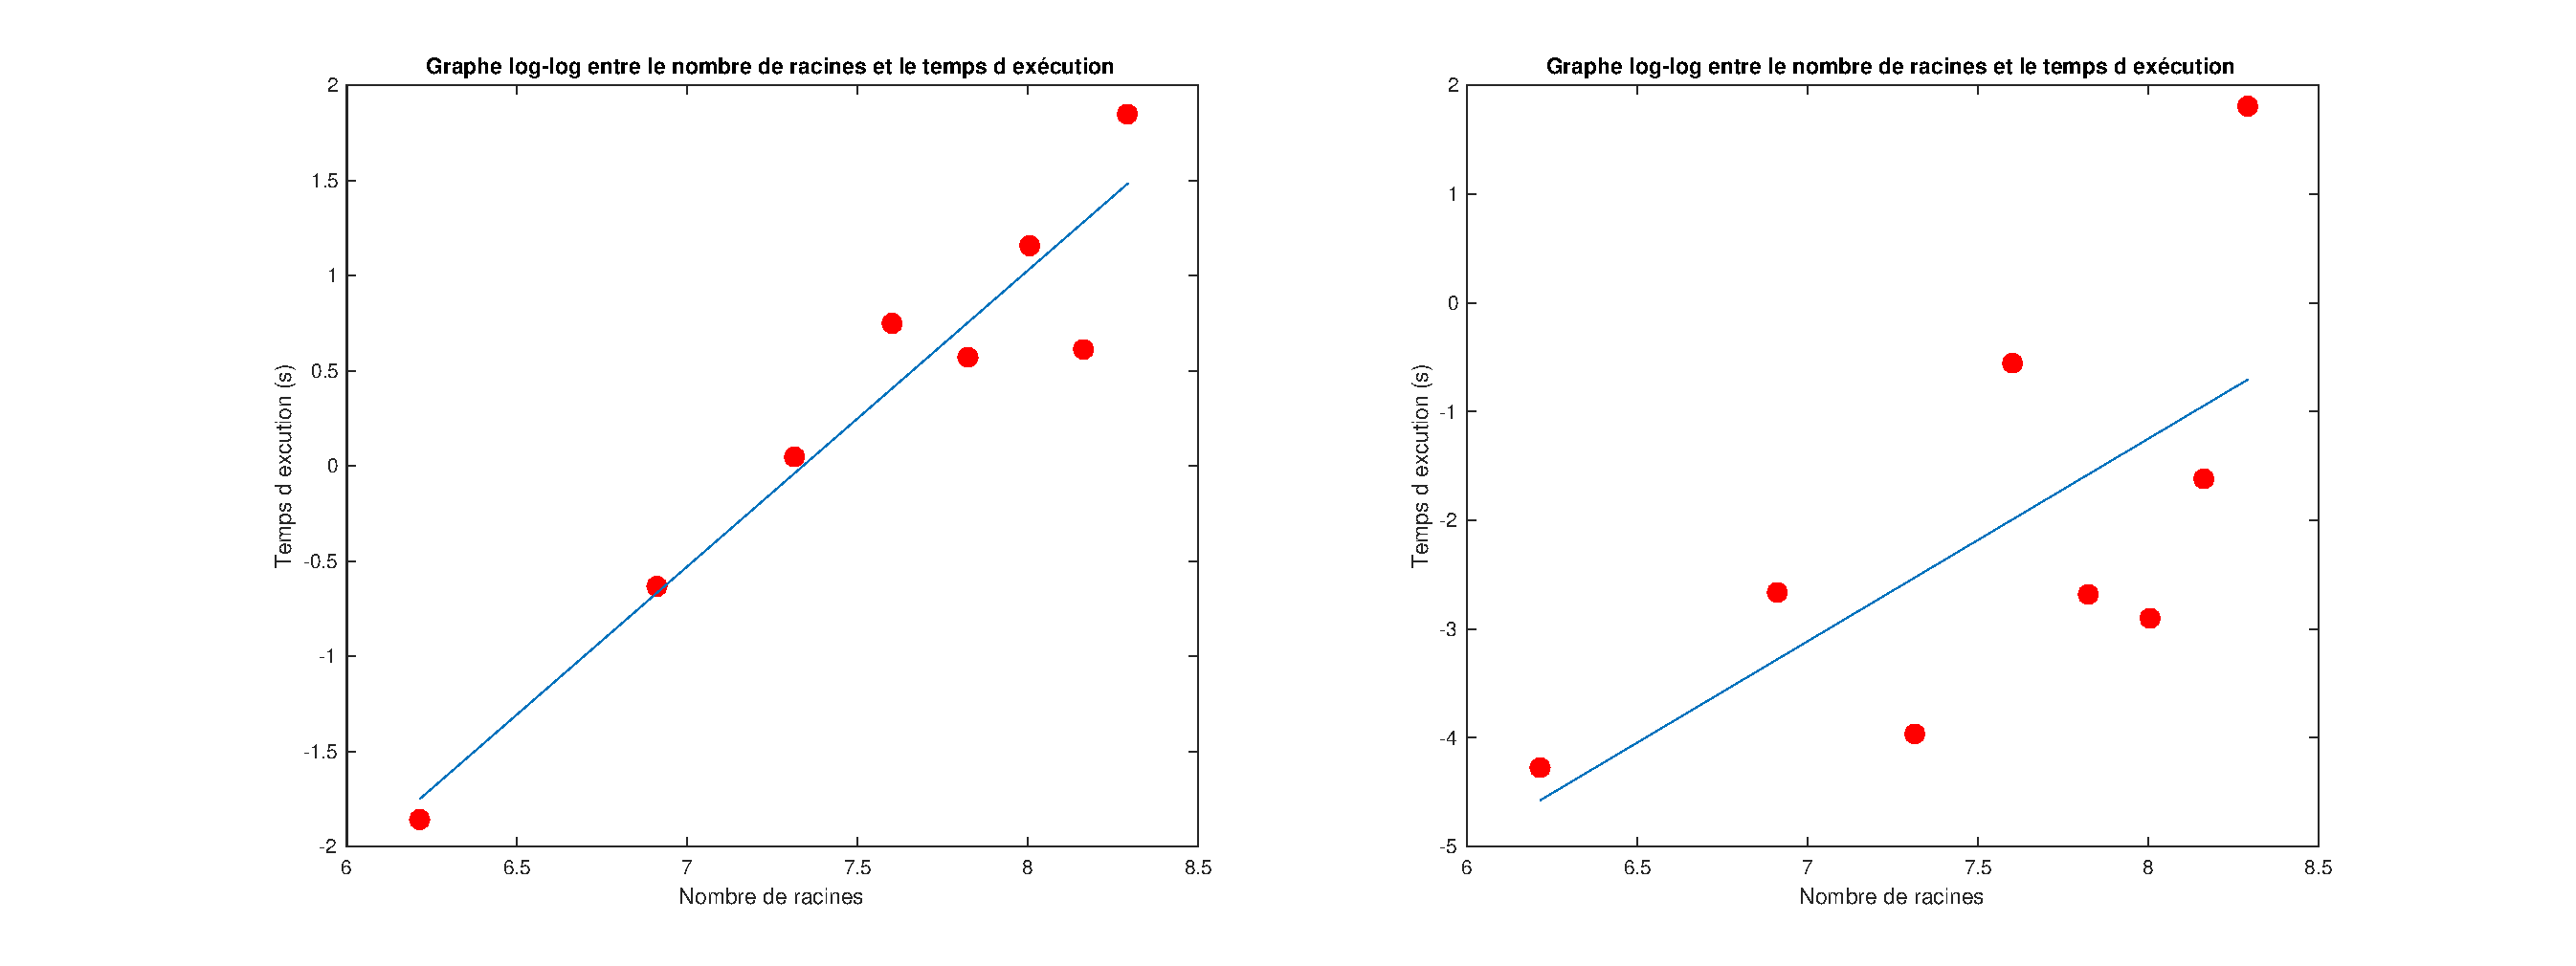
\includegraphics[width=15cm]{image/perfEucl}
        \end{center}

        Après expérience nous observons une complexité de $\mathcal{O}(n^{1.55})$ pour le cas de gauche et de $\mathcal{O}(n^{1.86})$ pour le cas de droite.
        Il faut noté que la complexité obtenue théoriquement est celle du pire cas ($n$ divisions euclidiennes nécessaires) et non celle du cas moyen, ceci peut donc
        expliquer nos valeurs expérimentales plus faibles.

\paragraph{Complexité de roots.m}
    Pour étudier la complexité de roots, nous avons mesuré son temps d'exécution en fonction du degré n de $f_0$.

    \begin{center}
    \begin{tabular}{|l|l|l|l|l|l|l|l|l|}
    \hline
        Degré de $f_0$  & 500 & 1000 & 1500 & 2000 & 2500 & 3000 & 3500 & 4000 \\
    \hline
       Temps d'éxécution (s) & 0.31 & 1.4   & 3.69 &   6.71  & 11.2  & 20.06  & 30.23 &  47.17\\
    \hline
    \end{tabular}
    \end{center}

    A nouveau, nous avons distingué deux cas : à gauche les coeffients sont entiers pris aléatoirement
    entre 0 et 10, à droite les coefficients valent 1. Ce second cas est moins bien conditionné et devrait prendre plus de temps.

    \begin{center}
      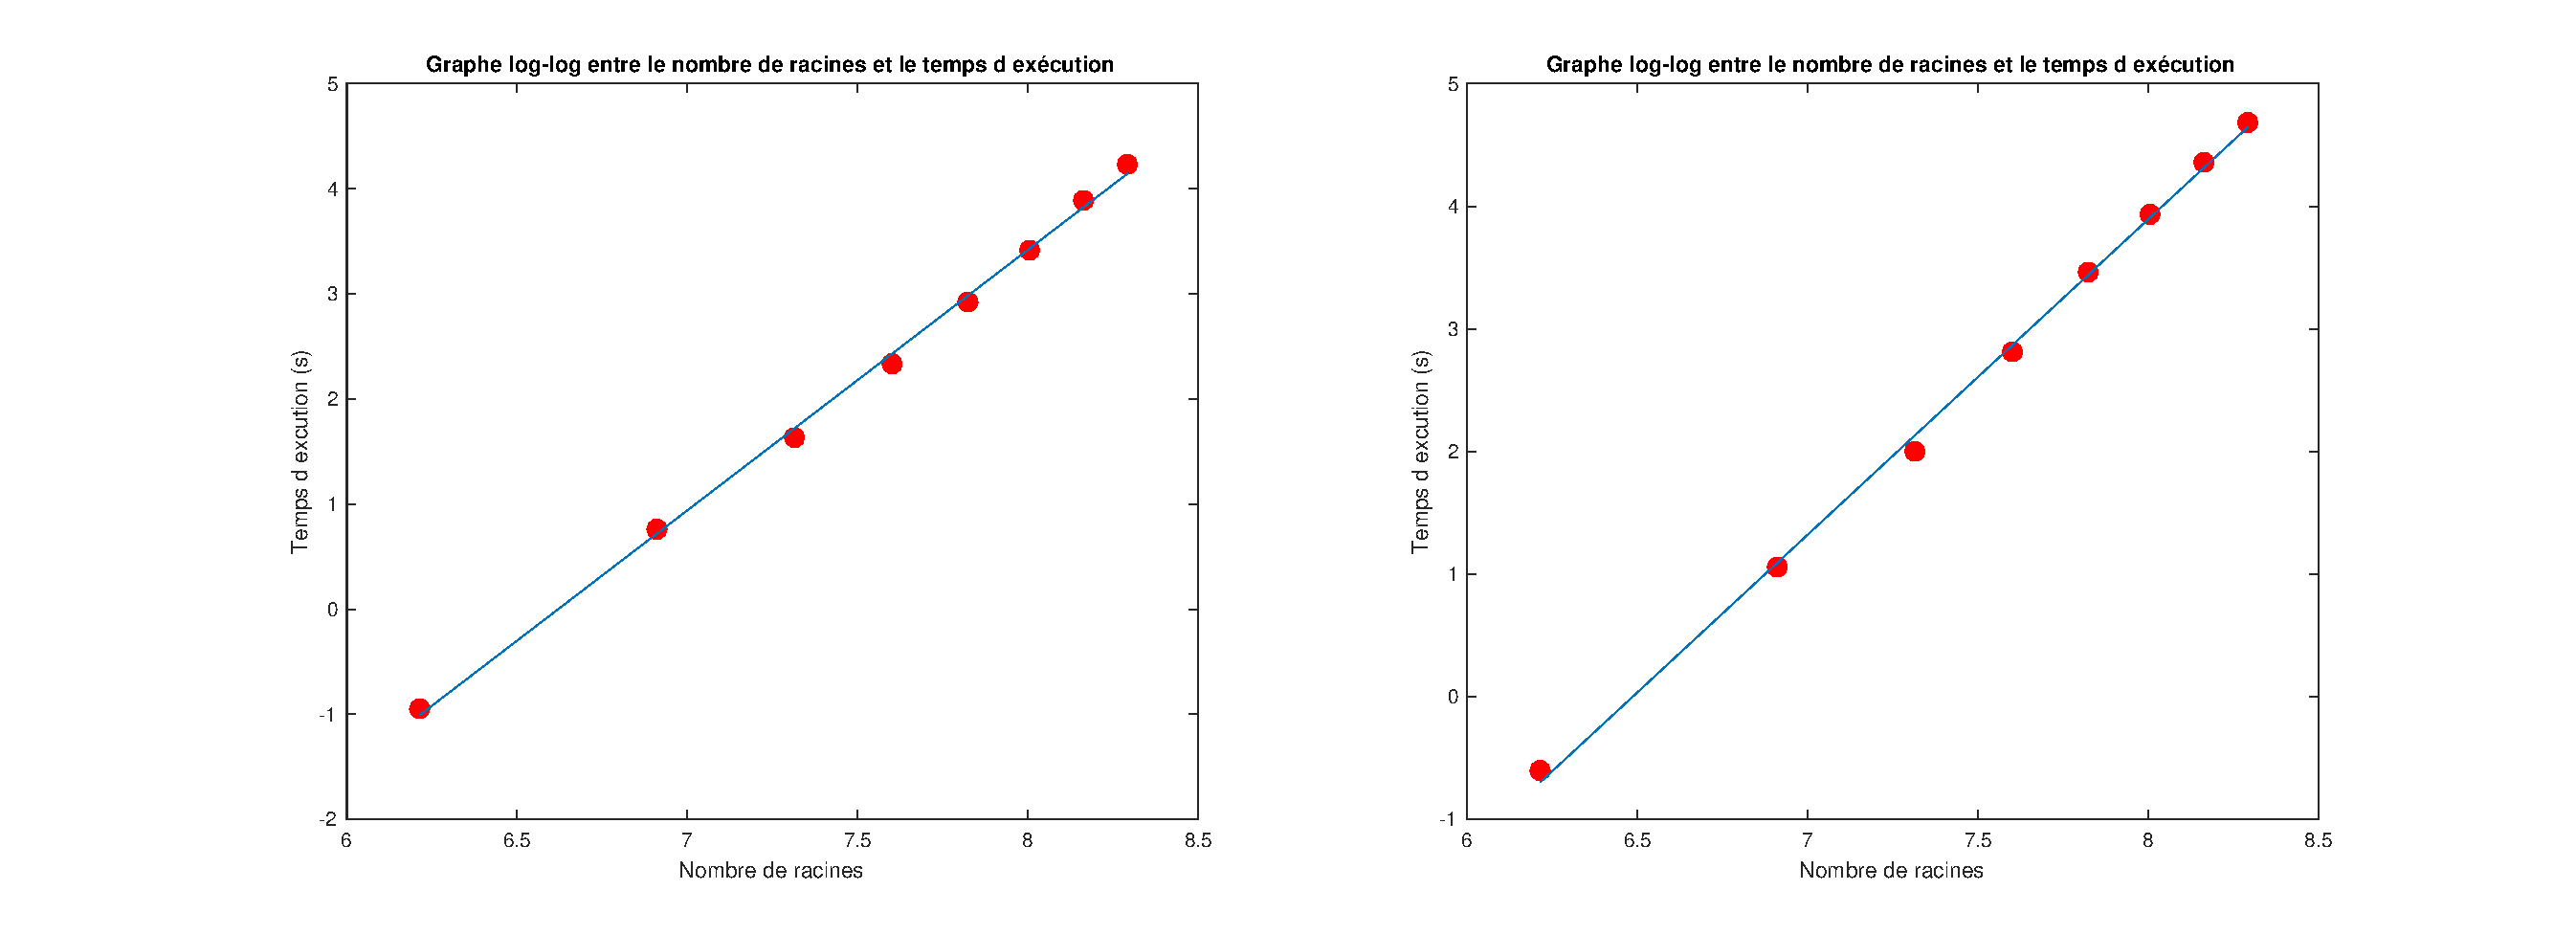
\includegraphics[width=15cm]{image/perfRootm}
    \end{center}

    Après expérience nous observons une complexité de $\mathcal{O}(n^{2.48})$ pour le cas de gauche et de $\mathcal{O}(n^{2.57})$ pour le cas de droite.
    Nous constatons également que la valeur théorique de 3 n'est pas atteinte. Nous imputons cette différence au fait que la complexité théorique est celle du pire des cas et que le notre, un polynome avec des coefficients unitaires\footnote{Un choix de coefficient aléatoire peut paraitre comme un choix plus pertinent, cependant il n'en est rien : comme le spectre des matrices de grandes tailles est en général assez homogène (valeurs propres suffisamment espacées), le problème est bien conditionné et le taux de convergence très rapide.}, n'est pas le pire.
\paragraph{Stabilité des fonctions}

\begin{itemize}
\item [\textbullet] AlgEuclide.m:
AlgEuclide renvoie pour n'importe quelle valeur de $\epsilon$ (même 0) le bon nombre de racines distinctes réelles (à savoir 2). Ceci est illustré sur la figure de gauche
de l'image ci-dessous.
    \item [\textbullet] root.m.:
        Le comportement de root.m renvoie les bonnes racines tant que $\epsilon > 10^{-30}$. En deçà de cette valeur, et jusque $\epsilon = 10^{-160}$, les racines restent justes, sauf celle sensée valoir $\epsilon$. L'évolution de cette dernière
        est représentée sur le graphe de droite de la figure ci-dessous. Idéalement nous aurions du avoir un évolution linéaire, hors nous voyons que lorsque epsilon tend vers 0, il y a un palier
        ce qui peut être expliqué par la limitation des nombres représentables dans Matlab.

        \begin{center}
          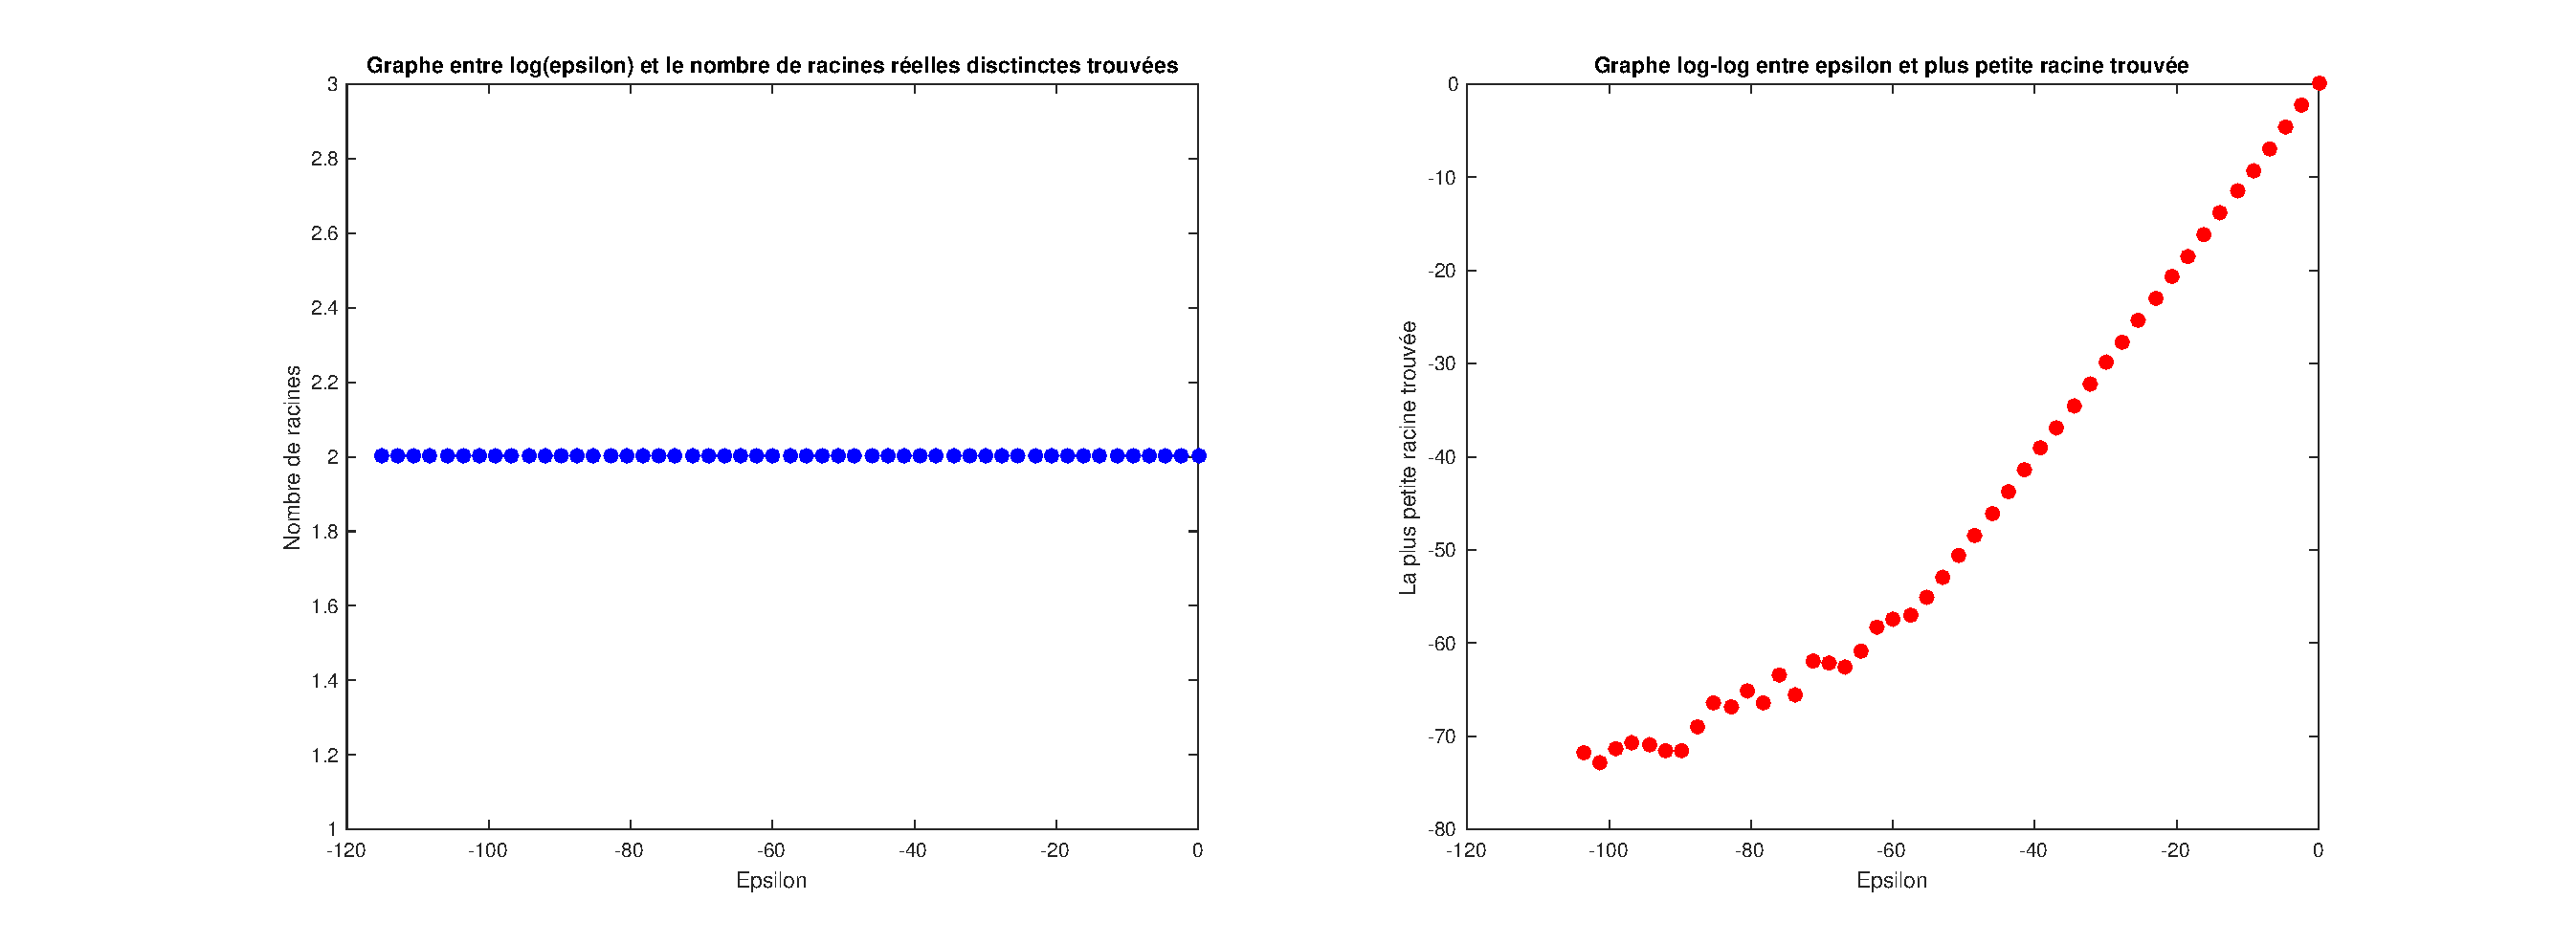
\includegraphics[width=15cm]{image/stab}
        \end{center}

\end{itemize}

\end{document}
